\begin{figure}[h!]
    \begin{center}
        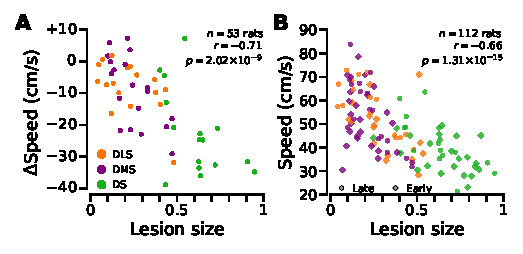
\includegraphics[scale=1]{ch-appendicies/figures/Speed.pdf}
        \caption[Speed-Lesion Size Correlation]
        {\textbf{The impact of the dS lesion on running speed correlates with lesion size.}
        \textbf{A)} Average change in running speed (speed after lesion~$-$~speed before lesion) versus lesion size, for all the rats that received a striatal lesion after training (late lesion).
        Running speed was calculated when rats crossed the treadmill from its back region to the reward area.
        All the running speed values obtained across 5 consecutive sessions were averaged to obtain the average running speed before (last 5 sessions before lesion break) and after (sessions \#4 to \#9, relative to lesion break) lesion.
        \textbf{B)} Average running speed versus lesion size for all the animals that underwent surgical lesion of the striatum.
        This dataset ($n=112$ animals) includes all the animals that underwent striatal lesion (DLS, DMS, DS) after extensive training (Late group, $n=53$, same animals as in panel~A), and animals that underwent lesion before training (Early group, $n=59$ animals).
        Speed was computed as in~A, except that average was done over the last 5 sessions (for both Early and Late groups).
        In four animals with a striatal lesion performed after learning the task (late lesion), the lesion size quantification could not be properly performed.
        These animals were classified according to their injection coordinates in the surgery (3 DLS and 1 DMS), however they were excluded from any analyses that required the lesion size (hence the difference between the number of ``late lesion'' animals in this figure, $n=53$, and the total number of animals in \autoref{fig:lesion:task}, $n=57$).
        }
        \label{fig:appendix:spd}
    \end{center}
\end{figure}